\chapter{提案手法}
\label{proposed}



\begin{figure}[hbtp]
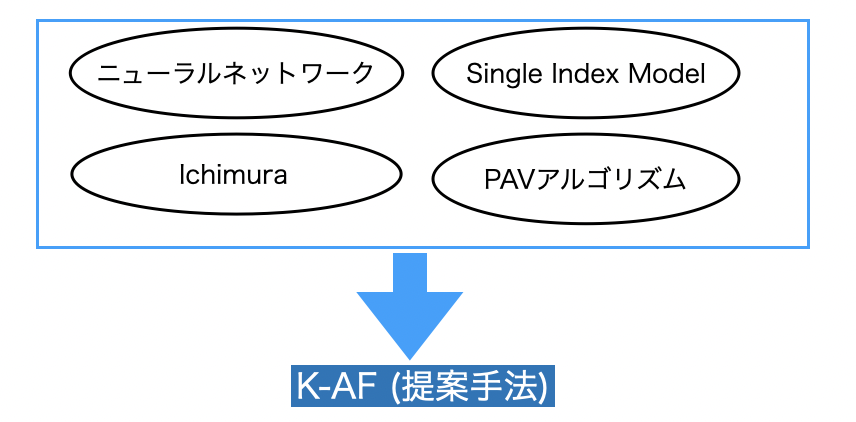
\includegraphics[width=15cm]{asset/proposed_method.png}
	\caption{提案手法}
	\label{proposed_method}
\end{figure}


本章では背景で述べた課題を整理しつつ、それらを解決する提案手法について述べる.
\ref{history_activation}では既存の活性化関数の動向を踏まえながら本提案手法へとつながる過程を述べる。
次の章で私が提案する活性化関数の数式について解説する。
次の章でそのアルゴリズムについて解説する。



\section{活性化関数と背景}
\label {history_activation}


\begin{figure}[hbtp]
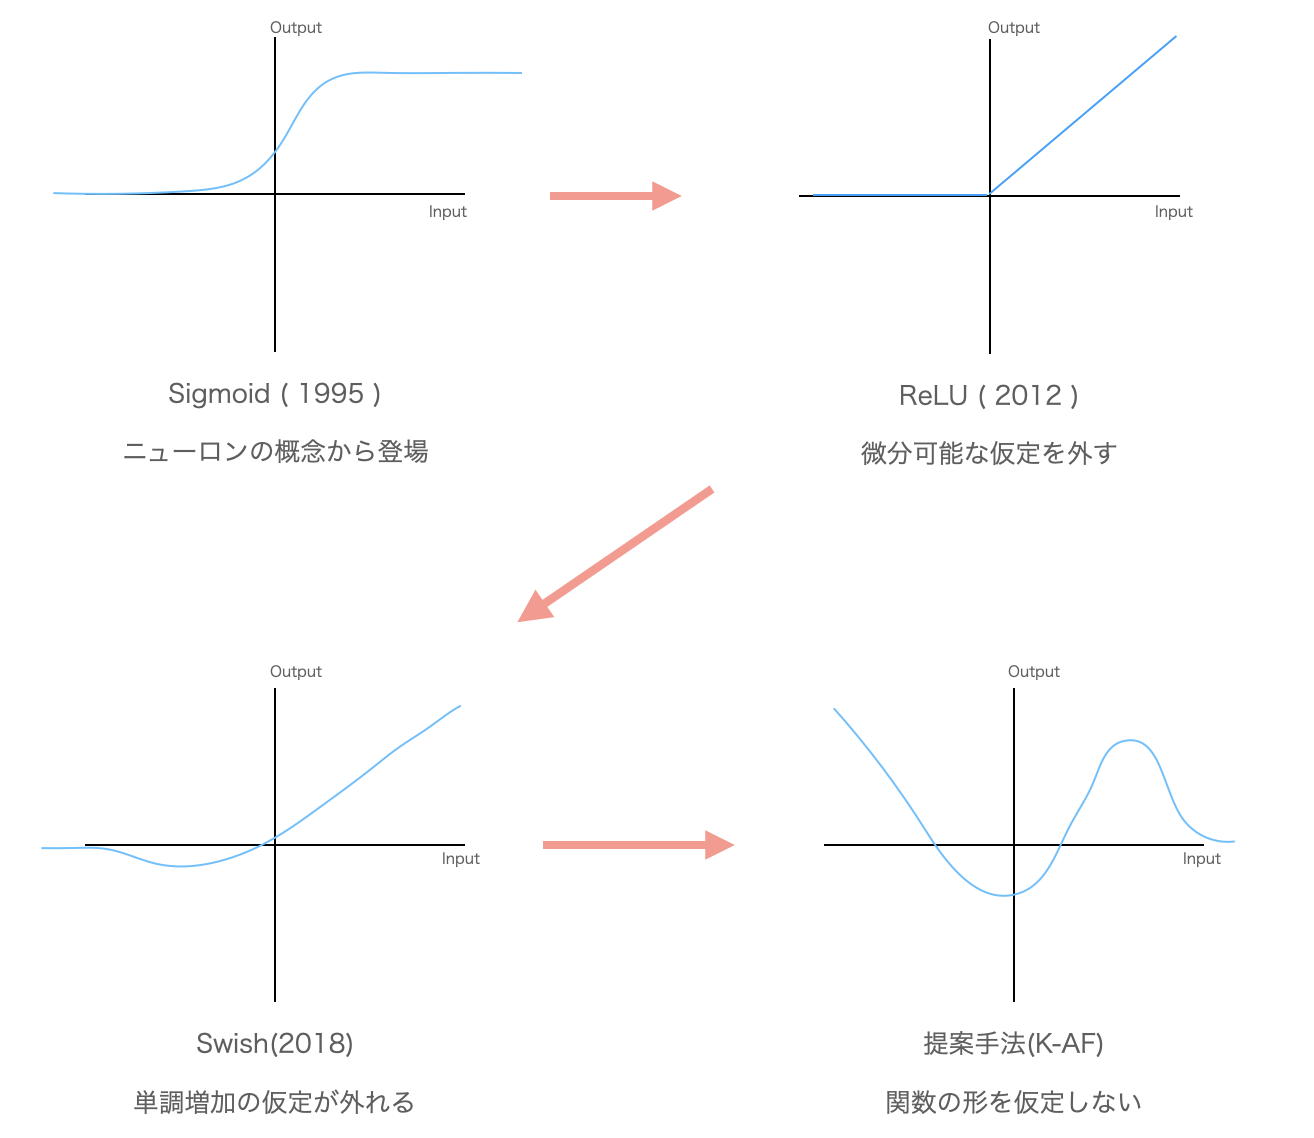
\includegraphics[width=15cm]{asset/history_af.png}
	\caption{活性化関数の歴史}
	\label{history_af}
\end{figure}

現在、深層学習に利用できる活性化関数が研究されている。特に近年では、中間層にReLUを用い出力層にSigmoid関数を用いた組み合わせがよく用いられている。
しかし、これらの組み合わせは経験的なものだけでなく、データに対する人間の知識が事前に必要とされる。

また、本研究はSwishやMishなどからの単調増加性の仮定を外した点に着目した。
ReLUやsigmoidといった関数はあくまでリンク関数の概念に相当していたこと考えると、
単調増加性というのは機械学習の観点では本来必要であったものかどうか問われるものであった。
統計学のSIMの法でも同様に単調増加性について仮定しているようであるが、本研究からはそれを外してやる。

そのため本研究ではSIMの考え方の中の単調増加性の過程を外し、本研究では、統計学の世界で使われているSIMのノンパラメトリック法を用いて、活性化関数に我々のリンク関数推定法を適用した。


そうすることで、より精度の高い結果を導き出すことができると予想される。
関数の形式はカーネル関数であり、入力の出力を一つの式で表現することができる。
これにより、深層学習に利用できる程度に計算コストを削減することができる。
また、今回の実験では、活性化関数を既存の関数から選択するのではなく、状況に応じた関数、つまり活性化関数の形を作ることができる。
そうすることで、関数全体から逆算して最適な関数を見つけることができる。これにより、これまでディープラーニングで課題とされてきた活性化関数の選択の問題を解決することが可能となり、新たなアプローチが可能になることが予想される。


\section{ノンパラメトリック}


現状ではディープラーニングに活かせるようなノンパラメトリックに推定する活性化関数は研究されておらず、経験的に中間層ではRelu、最終的なアウトプット層ではデータセットに合わせてSigmoidが使われることが多い。
しかしながらこれらの組み合わせは経験的であるだけではなく、データに対する人知見が事前に必要である。
本研究では、統計の世界で使われていたSIMでのノンパラメトリックな手法を用いて行われていたリンク関数の推定方法を活性化関数に応用する。
そうすることにより、経験的な知見による活性化関数の選択という行為を行わずともより高い精度の結果を導けるのではないかということである。
関数の形式はカーネル関数を用いることで、入力に対しての出力を一つの式で表せるようにする。そうすることでディープラーニングでも使えるぐらいの少ない計算コストが実現できる。


また、この実験により状況に応じた適切か活性化関数の形を既存のものから選択するのではなく、関数全体の中から逆算できると考えている。それにより、ディープラーニングの課題であった、活性化関数の選択問題という課題も新しいアプローチで解決できると考えている。




\section{カーネル密度推定}



本論文で私が提案する活性化関数を以下の数式で表現する。


\begin{eqnarray}
G(X_iw)=\frac{\sum_{i\neq j} K\left(\frac{X^{calc}_j w - X_i w}{h_{calc}}\right)Y^{calc}_j}{\sum_{i\neq j} K\left(\frac{X^{calc}_j w - X_i w}{h_{calc}}\right)}
\label{eq:k-af}
\end{eqnarray}

~\cite{ichimura}ではデータセットの数だけで表現していたが、一部を省略することにより少ない変数で表現することに成功した。



\subsection{バンド幅推定}
kernel関数は関数の形状を推定するにあたってバンド幅の大きさが非常に重要になる。

バンド幅は大きいほど関数の自由度が減り、小さいほど自由度が大きくなることが容易に推定できる。



\begin{figure}[hbtp]
    \begin{center}
        \begin{tabular}{c}
            \begin{minipage}{0.40\hsize}
                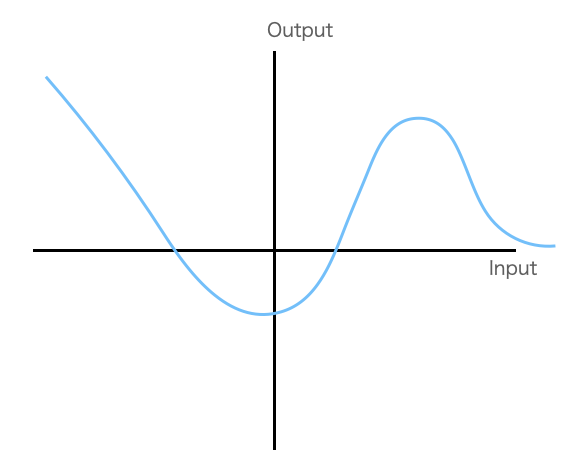
\includegraphics[clip, width=5cm]{asset/k_af_band_big.png}
                    \caption{バンド幅が大きいと、K-AFで表現できる活性化関数の数は減る。}
                    \label{k_af_band_big}
            \end{minipage}
            \hspace{10pt}
            \begin{minipage}{0.40\hsize}
                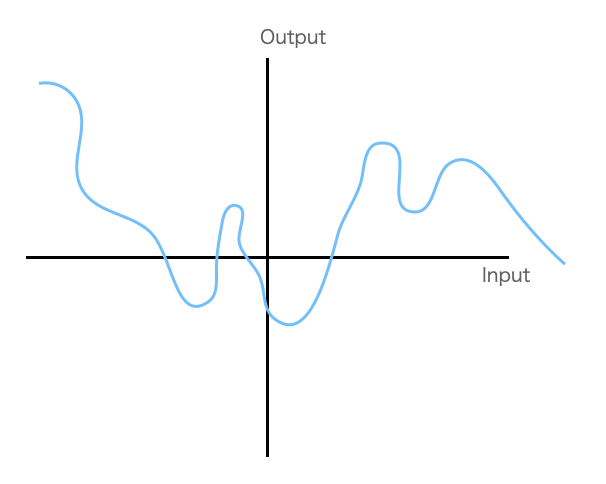
\includegraphics[clip, width=5cm]{asset/k_af_band_small.png}
                    \caption{バンド幅が小さいと、K-AFで表現できる活性化関数の形は大きくなる。}
                    \label{k_af_band_small}
            \end{minipage}
        \end{tabular}
    \end{center}
\end{figure}

\ref{k_af_band_small}の方が表現の幅が広いが、勾配消失の問題や過学習の問題が考えらる。
本実験ではこのバンド幅も学習のパラメータに含めることで最適なバンド幅を推定できるようにした。

\section{アルゴリズム}


\begin{algorithm}[]
	\caption{\KAF}
	\label{alg:fixed-u-alg}
\begin{algorithmic}
	\STATE {\bfseries Input:} data $\langle (x_i, y_i) \rangle_{i=1}^m \in
	\reals^d \times [0, 1]$, $u: \reals \rightarrow [0, 1]$.
	\STATE $w^1 := 0$;
	\FOR {$t = 1, 2, \ldots$}
	\STATE $h^t(x) := u(w^t \cdot x)$;
	\STATE $w^{t+1} := w^t + \displaystyle\fraconem \sumionetom (y_i - u(w^t
	\cdot x_i)) x_i$;
	\ENDFOR
\end{algorithmic}
\end{algorithm}

これが実装のアルゴリズムである。pythonでの実装についてはappendixで述べた。




%%% Local Variables:
%%% mode: japanese-latex
%%% TeX-master: "../bthesis"
%%% End:
